\documentclass[9pt,a4paper,]{extarticle}

\usepackage{f1000_styles}

\usepackage[pdfborder={0 0 0}]{hyperref}

\usepackage[numbers]{natbib}
\bibliographystyle{unsrtnat}


%% maxwidth is the original width if it is less than linewidth
%% otherwise use linewidth (to make sure the graphics do not exceed the margin)
\makeatletter
\def\maxwidth{ %
  \ifdim\Gin@nat@width>\linewidth
    \linewidth
  \else
    \Gin@nat@width
  \fi
}
\makeatother


% disable code chunks background
%\renewenvironment{Shaded}{}{}

% disable section numbers
\setcounter{secnumdepth}{0}

\setlength{\parindent}{0pt}
\setlength{\parskip}{6pt plus 2pt minus 1pt}



\begin{document}
\pagestyle{front}

\title{A computational reproducible manuscript}

\author[1]{Nelle Varoquaux\thanks{\ttfamily nelle.varoquaux@gmail.com}}
\affil[1]{a}

\maketitle
\thispagestyle{front}

\begin{abstract}
This is a fully computationally reproducible manuscript!
\# Archive statement:
All data (simulated data and code) is made available on GitHub. If accepted,
it will be archived with provided DOI in an appropriate scientific data
repositoriy.

\hypertarget{keywords-reproducibility-manuscript}{%
\section{Keywords: Reproducibility, manuscript}\label{keywords-reproducibility-manuscript}}
\end{abstract}


\clearpage
\pagestyle{main}

\hypertarget{introduction}{%
\section{Introduction}\label{introduction}}

This manuscript is an entirely computationnaly reproducible manuscript. The
code and the manuscript is contained in a git repository on GitHub. This git
repository is organized following the principles detailed in ``A quick guide
to organizing your computational biology project'' \citep{noble:quick}. The compiled
version of the manuscript can be found
\href{https://nellev.github.io/computationally-reproducible-manuscript/manuscript.pdf}{here}.
The Github repository containing the manuscript can be found
\href{http://github.com/NelleV/computationally-reproducible-manuscript}{here}.

\hypertarget{methods}{%
\section{Methods}\label{methods}}

Lorem ipsum dolor sit amet, consectetur adipiscing elit, sed do eiusmod tempor
incididunt ut labore et dolore magna aliqua. Ut enim ad minim veniam, quis
nostrud exercitation ullamco laboris nisi ut aliquip ex ea commodo consequat.
Duis aute irure dolor in reprehenderit in voluptate velit esse cillum dolore
eu fugiat nulla pariatur. Excepteur sint occaecat cupidatat non proident, sunt
in culpa qui officia deserunt mollit anim id est laborum

\begin{table}[htbp]
\centering
\begin{tabledata}{@{}lll@{}}
\header Name & Formula &\\
\row timely & \(\text{lfc}(t)\) & Function of time\\
\row abs\_sum & \(\sum_t \|lfc(t)\|\) & Always positive\\
\row max & \(\max_t \|lfc(t)\|\) & Always positive\\
\row min & \(\min_t \|lfc(t)\|\) & Always positive\\
\end{tabledata}
\end{table}

\textbf{Our data set is comprised of 300 samples in
2 dimensions.}

\begin{center}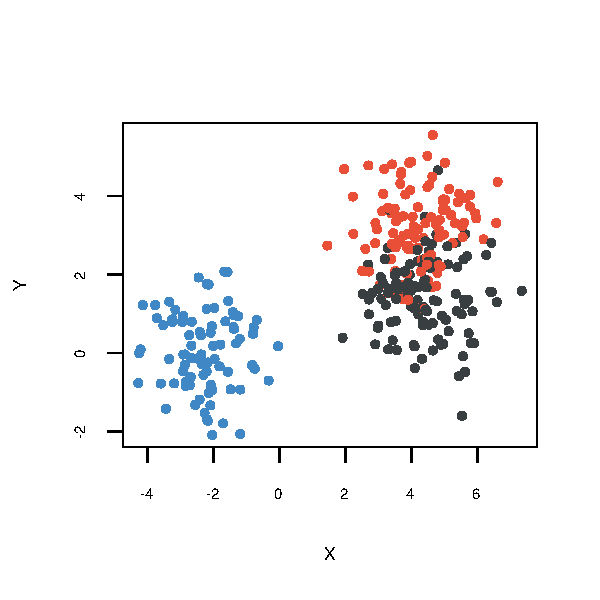
\includegraphics{/home/rstudio/repo/doc/reports/manuscript_files/figure-latex/plot_data-1} \end{center}

Lorem ipsum dolor sit amet, consectetur adipiscing elit, sed do eiusmod tempor
incididunt ut labore et dolore magna aliqua. Ut enim ad minim veniam, quis
nostrud exercitation ullamco laboris nisi ut aliquip ex ea commodo consequat.
Duis aute irure dolor in reprehenderit in voluptate velit esse cillum dolore
eu fugiat nulla pariatur. Excepteur sint occaecat cupidatat non proident, sunt
in culpa qui officia deserunt mollit anim id est laborum

\hypertarget{discussion}{%
\section{Discussion}\label{discussion}}

CQFD.

\renewcommand\refname{References}
{\small\bibliography{refs.bib}}

\end{document}
